\subsection{Kapselung Versatile
IKE Configuration Interface}
Wie erwähnt bietet strongSwan Open Source VPN Software das Versatile
IKE Configuration Interface (Vici) an, welche es erlaubt eine Management Anwendung über ein C, Ruby, Python oder Perl Binding an den Charon
IKE Daemon anzubinden.\\
Um die Vici Schnittstelle zu verwenden kann das passend pip Plugin installiert werden.
\\
\begin{lstlisting}[style=BashInputStyle]
	pip install vici==5.4.1dev3
\end{lstlisting}
\medskip
Um das Vici Plugin von unserem Code zu trennen, haben wir eine Wrapperklasse darum herum geschrieben. Dies verringert die Kopplung, ermöglicht uns eigene Exception zu werfen und gewisse Aufrufe zu kombinieren. \\
\begin{figure}[H]
\centering
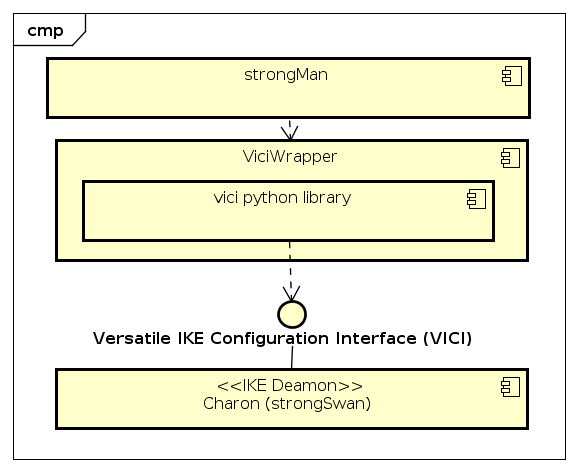
\includegraphics[width=250pt]{images/vici_wrapper.png}
\caption[Vici Diagramm]{Vici Diagramm}
\end{figure}
\medskip
Die Kommunikation, welche durch die Schnittstelle angeboten wird, basiert auf einem Unix Socket (AF\_UNIX). Dabei wird in Python die OrderedDictionary-Klasse verwendet, die als verschachtelte Property List für die Konfigurationsparameter dient. \footnote{\url{https://github.com/strongswan/strongswan/tree/master/src/libcharon/plugins/vici}}\\

\begin{python}
OrderedDict([
	('cert', OrderedDict([
		('remote_addrs', ['gateway'])
	)])
])
\end{python}
